\documentclass[a4paper,12pt]{article}
\usepackage{graphicx}
\usepackage{titling}
\newcommand{\subtitle}[1]{%
  \posttitle{%
    \par\end{center}
    \begin{center}\large#1\end{center}
    \vskip0.5em}%
}
\usepackage{url}
\usepackage[tight,footnotesize]{subfigure}  
\usepackage[top=2cm, bottom=2cm, left=4cm, right=2cm]{geometry}
\title{Processing GeoSpatial Data in BaseX}
\subtitle{Master Thesis in fulfillment of the requirements for the degree of
Master of Science (M.Sc.)}

\author{\\\\Author: \\
	Masoumeh Seydi
	\\\\\\Supervisors: \\
	Prof. Dr. Marc H. Scholl \\ 
	Dr. Christian Gr{\"u}n \\
	\\\\\\
	Konstanz University}

\begin{document}
\maketitle
\thispagestyle{empty}

\newpage
\section*{Abstract}

\thispagestyle{empty}

\newpage
\section*{Acknowledgments}
\thispagestyle{empty}

The completion of this master thesis would not have been possible 
without the support of many people. 
I must express my gratitude towards my supervisor 
Dr. Christian Gr{\"u}n for his continuous support and patience during my research.
I should confess that I can not imagine a better and friendlier
supervisor. Besides, I would like to thank also the other supervisor
Prof. Dr. Marc H. Scholl.

My sincere thanks also goes to Prof. ...  for
answering completely and accurately to many questions, asked
frequently. Finally, I wish to thank my parents for encouraging me 
throughout all my studies at University, and my best friend M. Ali Rostami.


\newpage
\tableofcontents

\thispagestyle{empty}
\newpage
\section{Introduction}
\setcounter{page}{1}
The geospatial data is increasingly becoming more important nowadays.
Different ways of processing this data is studied in ....

The time complexity ...

\subsection{Motivation}
BaseX~\cite{www/basex} is a high-performance XML~\cite{www/xml}
 database which is developed in Konstanz university.
It has a powerful text processor as well as the full support 
for XQuery~\cite{www/xquery,www/xqueryfun} language according to \cite{conf/xsym/GrunGHS09}.
Our goal is to empower BaseX to process the geospatial data in an efficient way.
Since BaseX is a XML database, this means to add the support of handling 
\emph{Geography Markup Language (GML)} data. The Open Geospatial Consortium (OGC)
which is an internationally recognized organization for geospatial standards,
is defined this new special XML grammer for the geographical data.
We want to have a complete support of this language in BaseX,
which means the abilities to read, to write, and to query on this data.


\subsection{Overview}
This essay will first define the concepts needed later in the discussion, called
Methodology, in Sec.~\ref{s.method}. In this section, the basic geospatioal data
and it's application areas will be introduced. Also, various ways that other works
are processing this data will be investigated in Sec.~\ref{s.rwork}. BaseX,
as a native XML database, which is our focus in this essay, is studies and extended
by a module to handle geospatial data in Sec.~\ref{s.basex}. 
Sec.~\ref{s.mongo} improves the efficiency of the module
by proposing another novel way considering MongoDB.
Finally, new ideas for further works are explained in
Sec.~\ref{s.future}.


\newpage
\section{Methodology}
\label{s.method}
According to \emph{Collins} dictionary, \emph{Geospatial} is an adjective relating to a position of things on the
earth's surface, also \emph{Geospatial Data}  is any data showing any thing on the earth's surface. Different 
countries and organizations are using different systems to represent this data. 
The World Geodesic System (WGS) is one of the standard system that is used world-wide 
for space-based satellite navigation system. \emph{WGS84} is the lateset version of this standard which
was introduced in $1984$. However, there are many different standards like ... and .... 
There are variuos convertors between ....

\subsection{Geospatial Data}
Geospatial data is the information describing features and locations  and their characteristics having a spatial component, which means are connected to a place on the earth. The entities are defined as geometries, i.e. points, lines, and polygons. The rules for uniquely identifying the position of geometries by an ordered set of numbers, called coordinates, are defined in the coordinate system. Since a geometrical figure could be described in different ways based on various requirements and definitions, there are numerous coordinate systems. A location could be defined with distinct coordinates from seprate coordinate system. In other words, various coordinates from different coordinate systems could point to the same location. Accordingly, it is necessary to know how they are related in concepts and definitions.

Geometry examples,
representing languages like gml,... and how we choose one!

Types of coordinate systems:
..............................


\subsection{Geospatial Data in Native XML Databases}
As a powerful XML grammer introduced by GIS community, \textit{Open GIS Consortium (OGC)}, \textit{GML} plays an important role in spatial data modeling, integration, sharing, transission, and exchange, beacuase of its flexibility in application schema, self-descriptive format, and rich data expression. Considering XML-based structure of GML, it could be perfectly handled in the native XML databases. ...

\subsection{General Spatial Requirements in Native XML Database}
In addition to general functions and features on XML structure of GML data, geospatial concepts and requirements could be included in the native XML databases. To start with, the GML format shouold be readed and treated as a Geometries. Therefore, just the string information is not enough to satisfy the geospatial features. In a target space with a set of geometries, the positions, locations, and relations of the geometries rises some requirements. For example, "What is the distance between two geometries?" Or, "Which geometries intersect this geometry?". Additionally, there are features related to single geometries, such as the lenght and area of a geometry, the number of interior ring of a polygon, and the start point of a line. Of course in a database the features related to a set of geometries are of more importane...................

\subsection{GeoSpatial Indexing}
According to \cite{survey}, indexing would dramatically influence efficient data manipulation and storage. Like any other type of data, geospatial data need to be indexed. Conventional index types are not suitable to support the spatial data, since the spatial data is very large and complex in structure and relations. Also, the operators used for data retrieval are complicated and spatial orderings would be hard to define. Another point which makes the traditional indices not suitable for spatial objects is that they would consider the spatial objects in one dimension and do not preserve the spatial proximity.

As it is examined in \cite{survey}, a large number of spatial indexes has been introduced to improve the spatial data retrieval.
The strength or weekness of an indexing approach mostly depends on requirements, query types, and applications. In the following sections, we go through selective spatial indexes based on three data structures Binary-tree, B-tree, and Quad-tree.

\subsubsection{Binary-tree Based}
The indexes in this group are basically and conceptually derived from the binary search tree. They adopt and generalize the idea of partitioning the space. Here some of them are explained.
\emph{The kd-Tree}.
This index, which was first introduced by Bentley \cite{bently1975}, is a binary search tree structure for organizing k-dimensional points. As it is explained in \cite{bently1975}, the basic idea is alternatively split the area by x- and y-coordinate, that at each level splits the points half in left, half in right, half below, and half above respectively. For every non-leaf node, there is a k-th dimension discriminator, which defines the the left and right subtrees order association with this node. If the discriminator is associated to the i-th dimension, all the i-th attribute of the sub-nodes in left subtrees are smaller than this node, and all the right sub-tree nodes have the i-th attribute greater.

\begin{figure}
\centering
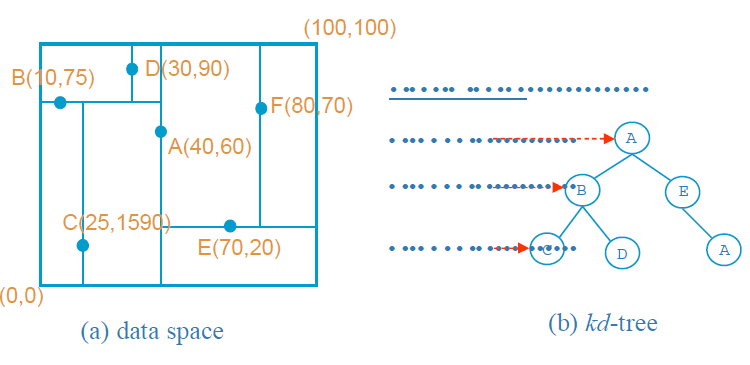
\includegraphics[width=0.5\textwidth]{kdtree}
\caption{kd-tree}
\label{figkdtree}
\end{figure}


When an item is deleted, a node from the sub-tree must be replaced. Here arises a complication that based on the discriminator in that level, let's call it i, either the node with the smallest i in right sub-tree should be replace or  the node with the biggest i in left sub-tree. A non-homogeneous kd-tree was proposed to make this process cheaper. 
Kd-Tree has been used a lot in intensive searches, but some variants has been introduced to make a better performance in clustering, searching, storage efficiency and balancing [survay], such as …..
and below we discuss some of them.

Main memory storage of the index trees are mostly a problem, since it is too big to be placed there  [survay]. Hence, the storage has to be done into disk space. Using binary search tree paging techniques [CeS82 survay] or tree organization of B-trees [BaM72 survay] to store the kd-Tree proposes new indexing structures.

Using properties of both kd-tree and B-tree [reference], the KDB-tree rebuilds the kd-tree to improve some inefficiencies of it.  It means benefits of the balanced kd-trees and the I/O efficiency of B-trees are together. It uses the disk space to bring the kd-tree on disk. 

The method which is used to build  KDB-tree is a space partitioning structure such that the partitions do not overlap each other. The partitions which stand for pages as organizational units, are organized in k-d-tree structure. 
KDB-tree has two basic structures: region page, consist of (region, pageID) pairs, and point page, consist of  (point, pageID) pairs. The region page contains the description of its subpages and a reference to those pages. The point pages contains actual data and references to them. 

\begin{figure}
\centering
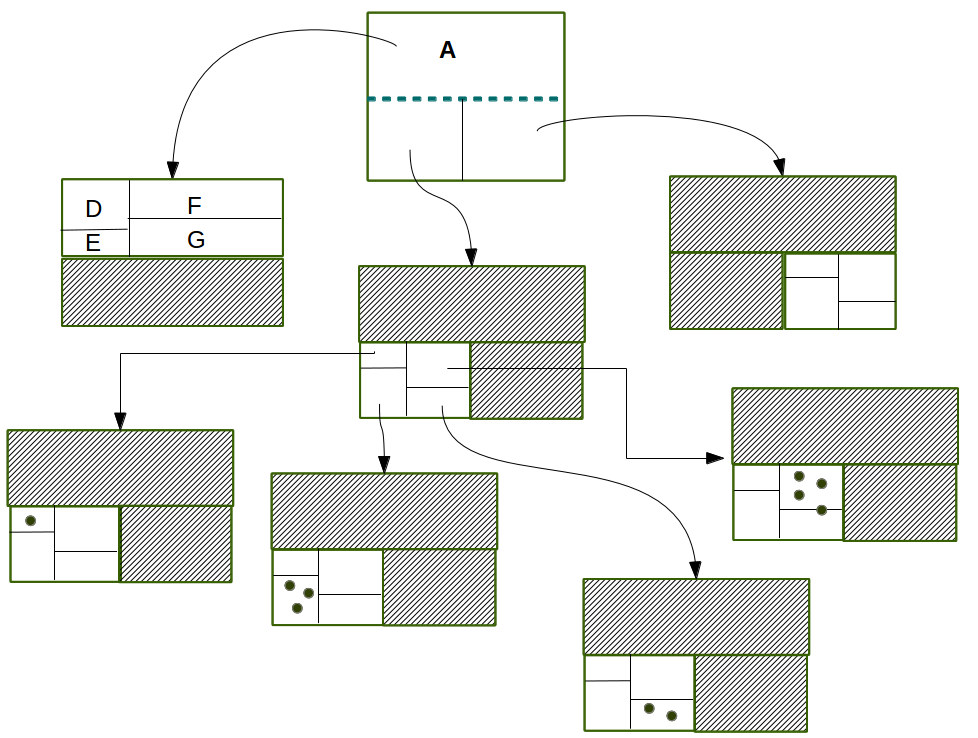
\includegraphics[width=0.5\textwidth]{kdbtree}
\caption{kdb-tree}
\label{figkdbtree}
\end{figure}

The pagination of the B-tree is integrated in the KDB-tree and consequently the tree is height-balanced. Space utilization and efficiency might be low or high, though, since the downward propagation of splitting, caused by region split, may cause low storage utilization. On the other side, there is no guarantee for minimum space utilization. Since partitions do not overlap, it is not always easy to find disjoint partitions to divide a region. So, those partitions must be split at the same value as parent, even though they do not use the minimum amount of space specified for each node. By this problem the range queries' performance is poor. 

Another variation of KDB-Tree which can be distinguished by two features: …
Since in a the region split in lower levels result in sparse nodes, hB-Tree (the holey brick Btree) as a multi-attribute index structure is proposed. Data spaces could be holey. It allows the data space associated with a node to be non-rectangular and it uses kd-trees for space representation in its internal nodes. The leaf nodes are known as data nodes and the internal node as index nodes. An index node data space is a union of its child node subspaces which are obtained through kd-tree recursive partitioning. It is height balanced since it is based on the K-D-B-Tree. 
Advantages of this structure is removing the sparse nodes of the K-D-B-Tree and reduction of search time and space utilization, since kd-tree is used. 
Disadvantages of this structure is that the deletion and splitting of nodes are expensive and also multiple references to a data node will lead to more than one traversal of a path.

\begin{figure}
\centering
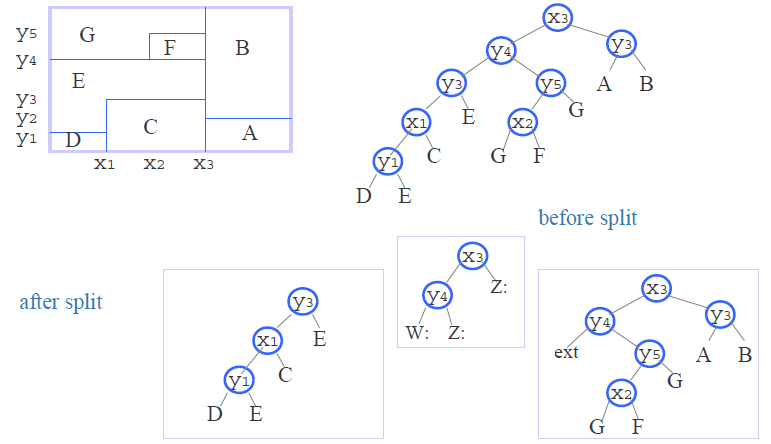
\includegraphics[width=0.5\textwidth]{hbtree}
\caption{hb-tree}
\label{fighbtree}
\end{figure}

\emph{Matsuyama’s kd-Tree}.
This structure is introduced for non-point objects and an extensive duplication strategy is used. The directory is a kd-Tree and a data page is associated for each leaf and those objects which overlaps multiple data spaces are identified in data page and also duplicates. Hence, the data page contains identifiers of the objects totally or partially contained in the corresponding data space.
The point is that this structure is not suitable for large objects since duplication and redundant storage of objects would result in high overhead.

\emph{4D-tree}
Indexes rectangular objects using kd-tree by mapping the objects into points in a four-dimensional space. Each 2D rectangle with (x1, y1) and (x2, y2) is considered as a 4D (x1, y1, x2, y2). As kd-tree the discriminators are chosen cyclically from this set. For each node, a discriminator, discriminator value and pointers to two children are stored. 
For a region search (qx 1, qx 2, qy 1, qy 2), depending on the discriminator, one of the x1 <= qx2, x2  >=  qx1, y1 <= qy2 or y2 >= qy1 has to be done to determine which subtree (or both) has to be searched.
The major problem associated with the 4-d-tree is its intersection search, which can be very costly due to the need for traversal of both subtrees when a query region lies in a subspace that cannot not bounded tightly using the discriminator values.

\emph{skd-tree}
The spatial kd-Tree alters the kd-tree in a way that objects are indexed by their centroid and the minimum bounding box of the object is also stored in the node. This structure is suitable for non-point spatial objects. In a kd-tree the objects which are contained in more than one space, will be referenced more than once. To avoid the duplication virtual subspaces are defined which include the original subspaces. So, each object are placed in the subspace based on its centroid.
With this devision, we just need one more value for each subspace which shows min/max values along the dimension of the discriminator. Therefore, the structure of each node would consist of:
Two children
The discriminator and it's value
The max/ min value of objects left(LOSON)/right(HISON) subspaces along with dimension of the discriminator
The maximum/minimum value of LOSON/HISON the nearest virtual line which bounds the data whose centroid are inside the LOSON/HISON.

\begin{figure}
\centering
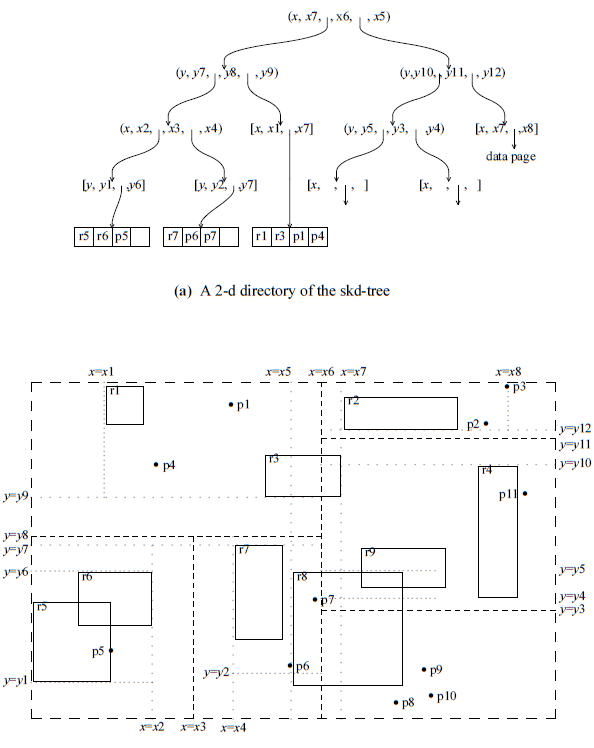
\includegraphics[width=0.6\textwidth]{skdtree}
\caption{skd-tree}
\label{figskdtree}
\end{figure}

During traversal a rectangular space is associated with each node and materialized  such that is tested against the query region if it intersects the region. 
(Since the virtual boundary may sometimes bound the objects tighter than the partitioning line, the intersection search takes advantage of the existing virtual boundary to prune the search space efficiently. To further exploit the virtual boundaries, containment search which retrieves all spatial objects contained in a given query rectangle was proposed. During tree traversal, the algorithm always selects the boundaries that yield smaller search space. The direct support of containment search is useful to operators like within and contain. The search rapidly eliminates all objects that are not totally contained in the query region.)
The Sdk-tree is memory-based, not a disk-based, data structure, thus is not suitable for very large databases.

\subsubsection{B-tree based Indexing Technique}
\emph{R-tree}

Minimization of both coverage and overlap is crucial to the performance of R-trees.
\subsubsection{$R^*$-tree}
The $R^*$-tree is found to be more efficient than some other variants, and the R-tree using linear splitting algorithm is substantially less efficient than the one with quadratic splitting algorithm. In general, the R*-tree is an improvement over the R-tree at the expense of more expensive insertion.

This structure tries to reduce overlaps between directory rectangles and the area covered by a rectangle, in order to make better performance, since minimum overlaps leads to less number of branches to be traversed in queries and minimum coverage helps to decide on the paths to traverse on higher levels. 
R*-Tree does these optimizations with revised node split and also forced insertion which finds a better place for a node that its original place. In R-Tree insertion-build structure is highly suboptimal and insertion and deletion could improves the R-Tree dramatically.
 (Using the idea of reinsertion of the R-tree, Beckmann et al proposed a reinsertion algorithm when a node overflows. The reinsertion sorts the entries in decreasing order of the distance between the centroids of the rectangle and the covering rectangle and reinserts the first p (variable for tuning) entries. In some cases, the entries are reinserted back into the same node and hence a split is eventually necessary. The reinsertion will no doubt increase the storage utilization; but it can be fairly expensive when the tree is large. The R*-tree is found to be more efficient than some other variants, and the R-tree using linear splitting algorithm is substantially less efficient than the one with quadratic splitting algorithm. In general, the R*-tree is an improvement over the R-tree at the expense of more expensive insertion.)

\emph{The Buddy Tree}
(In comparison to previously proposed tree structures such as the K-D-B-tree, the buddy-tree guarantees a more efficient dynamic behavior.Moreover, indirect splits which cause low storage utilization and high insertion costs in the K-D-B-tree, are completely avoided. This structure is 
It avoids the downward splitting of the K-DB-tree, the overlapping problem of the R-tree and the dependency of structures upon the insertion of data. The buddy-tree generalizes the buddy system of the grid-file to organize correlated data efficiently, by bounding the data points tightly using the bounding rectangle concepts of the R-tree and organize the directory as in the R-tree. Like grid-files, the non-zero sized data have to be mapped into higher dimension.
An important feature of the buddy-tree is that it does not partition empty data space. Therefore queries, such as partial match queries, where the query region intersects with empty data space, can be performed much faster than by conventional structures partitioning the complete data space.
The following summarizes the design properties of the buddy-tree:
empty data space is not partitioned
insertion and deletion of a record is restricted to
exactly one path
no overflow pages
directory grows linear in the number of records
performance is basicly independent of the sequence of
insertions
efficient behavior for insertions and deletions
very high fan out of the directory nodes)

\emph{The Packed R-Tree}

In order to minimize storage space, coverages and overlaps in R-Tree, constructing a static tree is proposed. To make this tree, first the objects are ordered along a coordinate. The object with the minimum value then is chosen to find the M nearest objects to that one, and assigns them to a node. Here M is the maximum number of objects that are allowed in a page. This step is repeated until the whole objects are assigned to a node. The bounding box of the leaf nodes are higher level objects. These are also ordered and assigned to the nodes. The process repeats until the number of the remained nodes is less than M. If so, they are assigned to the root.
The main objective of the algorithm is to reduce the storage space, the coverage and overlap of rectangles, in order to improve the search efficiency.

\emph{R+-Tree}

This structure is a compromise between the R-tree and the K-D-B-tree, to solve the overlapping problem of covering rectangles. It has just some difference:

Nodes of an R+-tree are not guaranteed to be at least half filled.
 The entries of any intermediate (internal) node do not overlap.
 An object identifier may be stored in more than one leaf node.

The duplication of the objects in the tree avoids overlappings and consequently leads to less path traversals in point queries. 
On the other hand there is some disadvantages: it might be bigger that R-Tree as a result of duplications, and the construction and maintenance are more complex that R-Tree or other variants. 
Also, in insertion cases into the tree a case would happen that the covering rectangles of some entries can prevent each other from expanding to include the new object. In other words, some space ("dead space") within the current node cannot be covered by any of the covering rectangles of the entries in the node. If the new object occupies such a region, it cannot be fully covered by the entries. When a new object cannot be fully covered, one or more of the covering rectangles are split. This means that the split may cause the children of the entries to be split as well, which may further degrade the storage efficiency.
In performance study, in the comparison between R-trees and R+-trees, it is found that the R+-tree requires much more splits, especially for large data objects, but lesser splits for smaller data objects. 
In general, the query efficiency tests show that R+-trees perform better for smaller objects and slightly worse off for larger objects.

\emph{STR-tree}

\emph{Cell-tree}
The cell tree introduces a structure to overcome the overlapping bounding rectangle problems of R-trees and the "dead space" (empty space) problems of R+-trees. Partitioning is done in a recursive way, but not necessarily with rectangles. Instead, the regions are polyhedral, as bounding polygons. Subspaces do not overlap.  
\begin{figure}
\centering
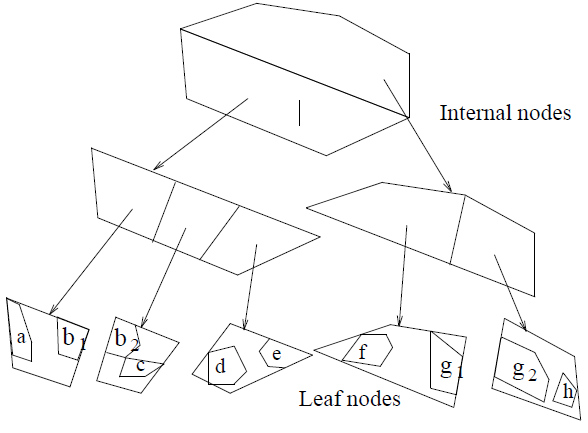
\includegraphics[width=0.5\textwidth]{celltree}
\caption{cell-tree}
\label{figcelltree}
\end{figure}

Like R+-Tree, objects might be represented in more than one leaf node. One problem with such an instruction which duplicates the objects is that each new object may be divided into multiple pieces in order to store them in a tree where internal node bounding polygons do not overlap. Specially in populated DBs. 
(Each split of a node leads to a decrease in the node data space but to an increase in the number of nodes per object. To overcome the fragmentation and duplication problems, Gunther and Noltemeier proposed to store oversized objects which may greatly increase the number of object identifiers being stored in the leaf nodes in separate "oversize shelves". These oversize shelves are data nodes linked to internal nodes in the cell-tree, in one way, causing the tree to be not height-balanced. The placement of a new object in the subtree or oversize shelf requires some optimization. The oversize page shelf can be overflowed and a split on this shelf is necessary.)
\emph{Quadtree}
It is organized in a way similar to the region quad-tree. A region is recursively partitioned until the resulting quadrants do not contain any rectangle. During the subdivision, all rectangles that intersect with either of the two partitioning lines are associated with the partitioning lines. The rectangles that are associated with a quadrant must not belong to any ancestor quadrant. It is assumed that no two rectangles overlap.
\newpage








\section{Related work}
\label{s.rwork}
Here, we are going to summerize a large set of literature over different methods
to store and process GML~\cite{gml} data. Section~\ref{storage} studies
different approaches to store GML. These approaches are investigated
with respect to the effectiveness of storage models in terms of query processing.
After the discussion over storage, the different proposed query languages
will be explained in Section~\ref{query}. Finally, we will look at the
famous databases in Section~\ref{s.dbs} and what they did to handle
GML data.
  
\subsection{Storage}
\label{storage}
One of the basic approaches to store GML data is proposed in \cite{Li2004}.
In this approach, the schema tree is generated at first. Then, the generated
tree is mapped to a relational schema to store all spatial objects as 
values of the mapped tables' field. Spatial query can be submitted 
in XQuery\cite{xquery}-like language with spatial functional extensions.
These GML queries are translated into equivalent SQL queries which are evaluated 
using spatial database management system.

Another similar approach is discussed in \cite{Zhu2011}. Here, GML is stored and queied 
focusing on non-schema documents. After the generation of the GML parse tree,
the nodes are analyzed and schema mapping is generated to store the doc in object-relational DB. 
Both spatial and non-spatial queries are supported in this approach.

Shulian Zhang et al~\cite{Zhang2008} considered both characteristics of XML DB 
and GML spatial data. Here, a native XML database based GML storage is proposed. 
A prototype system is developed on the basics of JAXP (Java API for XML Processing) program API 
and JTS~\cite{jts}, containing schema mapping constructor, document storage tool, 
and spatial analyzer.

\subsection{Query Languages}
\label{query}
XQuery language, recommended by \emph{W3C}, is only 
applicable to non-spatial data. To query spatial data in GML,
Fubao~\cite{Fubao2010} expanded the data model, algebra, functions, operations, 
and formal semantics in XQuery to achieve a GML query processor.
This processor deals with both non-spatial and spatial queries, 
and the results will be outputted in GML.
Supported data types are  Geometry, Coord, Coordinates, Point, LineString, LinearRing, 
Polygon, Box, GeometryCollection, MultiPoint, MultiLineString, and MultiPolygon.
Also, defined spatial operations are simple geometry operation, spatial relation 
operation, spatial analysis operation and specific geometry operation.
The operations are actually handled by JTS in background.

Beside GML is used to represent and exchange 
the geographic data, it also benefits its XML-based model in interoperability, 
and more importantly, could be queried. In \cite{corcoles2001}, the data model 
and algebra behind the language are based on a previously proposed model 
in which components and interrelations are represented as a directed graph. 
The vertices of this graph are geometry types and properties. The edges also
represent the element containment, relationship between elements, and values. 
This query language tries to provide an interface like SQL to work with GML.

Xia Li~\cite{Lisa2006} defines Xquery as a language  not sutable to query GML, 
since spatial related data types and semantics need to be treated different from XML. 
The purpose of this study is to define expand Xquery not for predefined GML elements, 
but more flexible.  A set of operators and functions on GML data types that cover 
the most typical queries over spatial data. The difference with the previous one is 
that this language is applicable not for predefined GML types, but to any type.

Chen~\cite{Chen2010} introduces a new integration of GML and Xquery. In this work,
spatial data types and operations are added to XQuery based on \emph{OGC Simple
Features Spesification} for \emph{SQL} to achieve GML spatial data query.
%Adding spatial data types 
%(Point, LineString, LinerRing, Polygon, MultiPoint, MultiLineString, MultiLinerRing 
%and MultiPolygon) and spatial operation functions (basic, relational, analysis,.. functions), 
%based on OGC Simple Features Specification for SQL, to XQuery can achieve GML spatial data query. 
%Moreover to the previous studies in this subject GML spatial data query language 
%based on XQuery, problem of GML spatial data query, reasons for extending XQuery to
%support GML spatial data query, features of GML spatial data query language, 
%content of XQuery spatial extension, architecture of GXQuery, implementation methods 
%of GXQuery, and query examples of GXQuery were detially studied and discussed. 
The following part of the code shows the idea. 

\begin{verbatim}
FOR $var1 IN doc(“CDUTCampus.gml”)//Building,
$var2 IN doc(“CDUTCampus.gml”)//Building
WHERE $var1/gml:name/node() = “CDUT Palestra”
AND $var2/gml:name/node() = “CDUT Gymnasium”
RETURN geo:Contains(geo:Envelope($var1), $var2)
\end{verbatim}

A semantic version of Xpath language is defined in \cite{Alemdros2011, Alemdros2013}, 
which is not based on the tree-based (syntactic) structure of the GML.
A system based on the semantic structure of GML is developed to store GML by PostGIS RDMS.
Then, Xpath queries are translated into SQL language, considering the GML schema
and the resulted query is represented in KML \cite{kml} in this system.

\cite{Gutierrez2004} A knowledge-based approach is used to querying heterogeneous spatial databases based on an ontology and conceptual and attribute similarities. The ontology, which may be independent of the databases, expands and filters a user query. Then, queries are translated into a formal specification of entity classes, which are compared against definitions in databases. This process is carried out by determining the conceptual similarity between entities in a user ontology and by comparing these entities in the ontology with entities in the conceptual models of databases. In addition, the specification of a query is done not only by identifying entity classes but also by considering constraints based on attribute values.

\cite{corcoles2004} Towards integrating spatial and non-spatial data, it's necessary to develop an integration sys. For querying the data in different sources. Here a prototype of a mediation system for querying XML spatial resources in GML is studied.  The main task of this approach is to provide users with a unique interface for querying spatial XML resources with different schemas, independently of their organization and location. It provides the infrastructure for formulating structured spatial queries by taking into consideration the conceptual representation of a specific domain in the form of an ontology. The resources are integrated using RDF. The most novel and critical feature of this approach is the querying of spatial XML resources, because it uses a different way from that of querying and relating non-spatial resources.

\cite{belussi2006} Base on the problem posed in different representation of spatial data in various resources ( For example, one dataset M1 may represent roads and bridges as regions, another dataset M2 may represent roads as regions and bridges as lines, a third dataset M3 may represent both as lines), or even in integration scenarios or architectures, a possible solution is to introduce some mechanism of query relaxation, by which approximated answers are returned to the user. In this study, the relaxation problem for spatial topological queries is considered. In particular,  some relaxed topological predicates are presented and is show in which application contexts they can be significantly used. In order to make such predicates effectively usable, the way that GQuery, an XML-based spatial query language, can be extended to support similarity-based queries through the proposed operators is also discussed.

\begin{verbatim}
Determine all roads overlapping some bridge.
for $x in document(bridge.xml), $y in document(road.xml)
where overlap($x/geometry, $y/geometry) = true
return $x

Determine all roads overlapping some bridge, up to a 22% error.
for $x in document(bridge.xml), $y in document(road.xml)
where overlap($x/geometry, $y/geometry,R,L,0.22) = true
return $x 
\end{verbatim}

Finally, a novel approach is propsed by Corcoles~\cite{corcoles2003} to integrate Geospatial data on the Web.
This data is stored and queried using GML format and a special query language. 
An ontology is used to solve the semantic heterogeneity of different GML documents.

\subsection{Geospatial Data in Well-known Databases} ??
\label{s.dbs}
Besides analysing some ideas in the field of geospatial processing in databases, 
it would be useful to see the geospatial features and functionalities in similar database systems 
In this section, geospetial issues in three well-known databases, MongoDB, eXist, MarkLogic 
are explained to see how the different ideas are being provided and being used in practice. These database are 
selected since they are new in this filed and also all having geospatial functionalities. 


\subsubsection{MongoDB}
\label{mongo}
\cite{mongogeneral2010}
\cite{mongoinaction2011}

Geospatial Index:

There is two special indexes in MongoDB: 2d indexes that uses planar geometry when returning results and 2sphere indexes that use spherical geometry to return results.

When an index is created, geohash values for coordinate pairs are calculated and then the geohashes are indexed.
Geohash is calculated by recursively dividing the a 2D map into quadrants and assigning each area a 2-bit value.


If the file contains just flat data, the 2d Index has to be used, but for those which also contain spherical data, 2sphere Index has to be chosen, since the distance function differs respectively.

Later on geohash values will be index using B-Tree. 
MongoDB also used B-Tree structure for other type of index, such as Single Field (e.g. indexing over names), Compound, Text Index. (Probably this point effect on the structure of geospatial index.)

Geospatial Functions:

geoWhithin, near (flat space), nearSphere (spherical space), geoIntersect, which could be mixed with other non-spatial functions (like find, ...). 
centerSphere (for spherical space), center (for flat space, define a circle with a specified radius), maxDistance (mixed with near functions to specify the demanded distance), box (defines a box, could be also mixed with geowithin function), polygon (defindes a polygon), inqueDocs (to prevent a through put a document twice in query results)

\begin{figure}
\centering
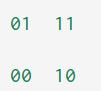
\includegraphics[width=0.1\textwidth]{mongoformat}
\caption{MongoDB Format}
\label{fig}
\end{figure}

mongoformat

Geohash (wikipedia)
Geohashes offer properties like arbitrary precision and the possibility of gradually removing characters from the end of the code to reduce its size (and gradually lose precision).
As a consequence of the gradual precision degradation, nearby places will often (but not always) present similar prefixes. Conversely, the longer a shared prefix is, the closer the two places are.
The main usages of Geohashes are
as a unique identifier.
represent point data e.g. in databases.
When used in a database, the structure of geohashed data has two advantages. First, data indexed by geohash will have all points for a given rectangular area in contiguous slices (the number of slices depends on the precision required and the presence of geohash "fault lines"). This is especially useful in database systems where queries on a single index are much easier or faster than multiple-index queries. Second, this index structure can be used for a quick-and-dirty proximity search - the closest points are often among the closest geohashes.
One limitation of the Geohash algorithm is in attempting to utilize it to find points in proximity to each other based on a common prefix. Edge case locations close to each other but on opposite sides of the Equator or a meridian can result in Geohash codes with no common prefix.[1]
Secondly a geohash essentially defines a bounding box within which a location lies, therefore two locations may be spatially very close but have different geohashes. In order to be useful to proximity searches, the surrounding eight geohashes of a geohash must be calculated and the locations matching these pulled out, therefore complicating potential usage in proximity searches.

\subsubsection{MarkLogic}
Geospatial data is marked up in XML elements and/or attributes. MarkLogic could handle and query different formats, such as GML, KML, GeoRss, and even general format for geometric data which are not based on a specified format. Only WGS84 and Raw coordinate systems are supported. WGS84 is used for data on the earth geometry, and raw coordinate system is suitable for data on flat plane.

Regarding the geospatial queries, the following types are supported:
\begin{itemize}
\item point query--matches a single point
\item box query--any point within a rectangular box
\item radius query--any point within a specified distance around a point
\item polygon query--any point within a specified n-sided polygon
\end{itemize}

Additionally, there are some Geospatial Operations as built-in functions to perform operations on geospatial data (in cts namepsace):

 box-intersects → Returns true if the box intersects with a region.
 circle-intersects → Returns true if the circle intersects with a region.
 polygon-intersects → Returns true if the polygon intersects with a region.
 complex-polygon-intersects → Returns true if the complex-polygon intersects with a region.
 polygon-contains → Returns true if the polygon contains a region.
 complex-polygon-contains → Returns true if the complex-polygon contains a region.
 distance → Returns the distance (in miles) between two points.
 shortest-distance → Returns the great circle distance (in miles) between a point and an region. The region is defined by a region.
 destination → Returns the point at the given distance (in miles) along the given bearing (in radians) from the starting point.


 XQuery Primitive Types And Constructors
These constructors (as functions from search module, cts namespace) are used in geospatial queries (cts:query constructors), defining regions as instances of cts:region, then the query returns true if the searching data are inside the region.
 cts:box 
 cts:circle
 cts:complex-polygon
 cts:linestring
 cts:point
 cts:polygon

 WKT

	WKT language also is supported for geospatial data representation. The parse-wkt function is used when WKT is used. It converts WKT to sequence of region items. Also, cts:to-wkt function could convert cts:region type in MarkLogic to WKT.

GeoSpatial Coordinates and Regions in MarkLogic Server


Latitudes and longitude pairs shape point. Points shape other geometries, like circle or polygon. Boxes are formed by 4 points which on the surface of the Earth, the edges of the box are arcs, but when those arcs are projected into a plane, they become two-dimensional latitude and longitude lines, and the space defined by those lines forms a rectangle.


The Geospatial Index
It is not based on quad or R-tree. It works like a range index with points as data values. In this range index, every value is a pair of latitude and longitude. Like an array of x,y values, sorted mainly based on lat and then long values. The values in array also are connected to the corresponding doc.
The points would be founded easily in a sorted structure. Boxes could be found first by finding the lat range, then checking for the long range. For circles and polygon as more complex ones, the bounding box is used to find the region they belong to. Also, to check if a point is inside the polygon, the number of intersections with the northward or southward arc of the point is counted. 

…. 

Different types of Geospatial Indexes: (???)

 Geospatial Element Indexes: data is represented by whitespace or punctuation separated element content 
 Geospatial Element Child Indexes: data comes from whitespace or punctuation separated element content, but only for elements that are a specific child of a specific element.
 Geospatial Element Pair Indexes: data comes from a specific pair of elements that are a child of another specific element.
 Geospatial Attribute Pair Indexes: data comes from a pair of specific attributes of a specific element.
 Geospatial Path Range Indexes: data is expressed in the same manner as a geospatial element index and the element or attribute index is defined by a path expression.


Geospatial Index Positions
	For each geispatial index there is a positions options, which is used for queries with restrictions of data distance inside the document.

Geospatial Lexicons1
Provided by spatial index, containing unique values of  geospatial data. 

“geo” Xquery Library
geo:box
Create a cts:point value from an element representing a box in one of the supported markup vocabularies.
geo:circle
Create a cts:circle value from a radius and an element representing a point in one of the supported markup vocabularies.
geo:geospatial-query
Returns a cts:query matching points within given regions.
geo:geospatial-query-from-elements
Returns a cts:query matching points within given regions.
geo:interior-polygon
Create a sequence of cts:polygon values from a polygon element in one of the supported markup vocabularies.
geo:point
Create a cts:point value from an element representing a point in one of the supported markup vocabularies.
geo:polygon
Create a cts:polygon value from a sequence of point elements in one of the supported markup vocabularies.


“gml” Xquery Library
gml:box
Create a cts:box value from a GML Envelope element.
gml:circle
Create a cts:circle value from a radius and GML Point element.
gml:geospatial-query
Returns a cts:query matching points within given regions.
gml:geospatial-query-from-elements
Returns a cts:query matching points within given regions.
gml:interior-polygon
Create a sequence of cts:polygon values from a GML Polygon element.
gml:point
Create a cts:point value from a GML Point element.
gml:polygon
Create a cts:polygon value from a sequence of GML Point elements or a GML Polygon element.


“geoRss” Xquery Library
georss:circle
Create a cts:circle value from a radius and GeoRSS point element.
georss:geospatial-query
Returns a cts:query matching points within given regions.
georss:point
Create a cts:point value from a GeoRSS point element.

“kml” Xquery Library
kml:box
Create a cts:point value from a KML LatLongBox element.
kml:circle
Create a cts:circle value from a radius and KML Point or Location element.
kml:geospatial-query
Returns a cts:query matching points within given regions.
kml:geospatial-query-from-elements
Returns a cts:query matching points within given regions.
kml:interior-polygon
Create a sequence of cts:polygon values from a KML Polygon element.
kml:point
Create a cts:point value from a KML Point or Location element.
kml:polygon
Create a cts:polygon value from a KML polygon or a sequence of KML Point or Location elements.


“cts” Functions
Part of these functions also contain geospatial function: 1 2
----------------------------------------------------------------------------------------------------------------------------
For querying on geospatial data, after loading the data into the DB and making the indexes, primitive types should be constructed to be used in the geospatial cts:query functions. Then, geospatial queries needs to be constructed, using primitive types. 
Also, there are modules to convert the Metacarta, GML, KML, and GeoRSS formats to cts:box, cts:circle, cts:point, and cts:polygon formats, to pass them into the cts:query constructors and make appropriate queries.

\subsubsection{eXist-db}
The design if spatial index in eXist-db doesn't store character data from the document. It stores WKB index entries in a JDBC database, namely a HSQLDB. In other words, the spatial data is stored in the DB, but geometries, as JTS Geometry instances, are held in memory, waiting for a special mode to be flushed into a relational DB, insertion or removal. The Geometry WKT would be serialized and deserialized to and from the database.
The index is made by the relational db (uses an SQL database to index spatial data) and the geometric functions are applied using JTS library.



Both PostGIS and Oracle Spatial share the same “R-Tree” [1] spatial index structure. R-Trees break up data into rectangles, and sub-rectangles, and sub-sub rectangles, etc. It is a self-tuning index structure that automatically handles variable data density and object size.

Ideas

Query general format geospatial data, considering the data as a set of points, ...
Storing the eospatial data in geohash ???
…


\subsection{Others}
\newpage

















\section{Spatial Querying in BaseX}
\label{s.basex}
%TODO tozihe bishtar dar more requirements va inke chera injuri develop shode
Spatial query is a spacial type of query with two certain properties in general. First, they use geometris as inputs and in some cases as ouputs. Ofcourse, in XML databases geometries are expressed in XML sructure, like GML elements. Moreover, they consider spatial relations between the geometries. 
Regarding the related works and ideas in ?????, there are various viewpoints in providing geospatial features in a database up to some extend of requirements fulfillment. Following the Open Geospatial Consortium (OGC) Simple Feature (SF) [????] data model, geospatial features in BaseX follow the EXPath geospatial API function interface specification which defines commonly used and implemented function signatures from the Open Geospatial Consortium Simple Features Common Access API version 1.2 \cite{simpleFeature}. Since the OCGSF data model typically will be representeg in GML, the idea has been started to develope in BaseX to support GML format. However, an implementation would support the other encodings, like KML. 

In this section, we explain \textit{Geo Module} in BaseX in which the geospatial functions are introduced and the the implementation details, which would be starting point for furthur developments. Moreover, indexing and the related time complexities are discussed in the following, as the critical issue in this thopic.

\subsection{Geo Module in BaseX}
As mentioned above, geospatial features in BaseX are implemented based on the EXPath Geo Module Specification \cite{expath}. The specification contains the difinition of functoin for widely used geographic and geometric analysis operations, from Open Geospatial Consortium Simple Features Common Access API version 1.2 \cite{simpleFeature}. The functions apply to geometries in different formats, such as GML, KML, GeoJSON, Well Known Text (WKT), and even Well Known Binary (WKB). Based on the specification, \textit{Geo Module} in BaseX comprises a set of functions, such as intersection, within, distance, boundary, centroid, diference, union, and etc., added to the “basex-api” package in BaseX. In addition, geospatial index structure is implemented in BaseX core. The geometries supported in this module are Point, LineString, Polygon, plus MultiPoint, MultiLineString, and MultiPolygon. The module is an individual package with a set of classes as briefly described bellow,
\begin{itemize}
\item Geo: This class is the main class, in which all geo spatial functions are defined and implemented and are used in Xquery.
\item GeoError: Ths class defines error functions with related massages to be thrown.
\item GeoTest: Contains functions to test the functions implemented in \textit{Geo.java} class.
\item GmlReader: Functions required to read the GML geometries as xml elements are implemented in this class.
\item GeoIndex: Functions to use geo spatial index in geo functions and queries are implemented here. 
\end{itemize}

Spatial indexing and related implementation details will be described in the next section. Here we explain general functionalities of this module.

The geospatial functions, defined as public in \textit{Geo.java} class, are accessible from BaseX GUI, as defined in the specification. They use some private functions to read geometries or write them out into the GUI. Besides, each function uses corresponding function from JTS library[ref.????] to do the required geometric operation and provide the appropiate result. Here we briefly explain the process by which the input geometries, either from a variable or a database node, is processed and the result is returned.
Let's start it with an example, asking for geometries within a specified polygon (\$p). The query should be written using Xquery via BaseX GUI as follow,

\begin{verbatim}
let $p := 
<gml:Polygon>
  <gml:outerBoundaryIs>… </gml:outerBoundaryIs>
<gml:Polygon>
	
for $x in //gml:Polygon
  return if ( within($x, $p) ) then $x else ()
\end{verbatim}

Each geo spatial function has at least one geometry as input, like function “within” above. In this example, the \textit{\$p} variable is provided as a node and the \textit{\$x} variable is each \textit{<gml:Polygon>} node in the current database. To read the geometries in a node when the geo function \textit{within} is called, the private function \textit{geo} first checks the element name to make sure that at least the node name is a valid geometry name. It means, if the element name is something out of the set of geometry names, the function would throw an error. 
Then, the gmlReader class is used to read and pars the whole element and to check their validity based on GML 2.0 format. That means, geometries have to be formatted in GML 2.0 to be validated and analyzed for further operations. The reader is implemented as the \textit{GMLReader.java} class and differently reads the elements based on their types (tag names). If the element is a valid GML geometry, the function creates the corresponding geometry, using JTS constructors. Otherwise, the corresponding error massage will be shown. For instance, if a polygon does not have any outer ring or the coordinates of a geometry are not valid coordinates, an error will be thrown. 

(Figure for this process)

Now, the geometries are ready to be processed in a geometric operation, like checking two geometries whether they intersect each other, finding the symmetric distance of two geometries, and getting the number of inner rings of a polygon. The operation is done using the JTS function. The functions output could be in any XML Schema [???] data types, such as integer, boolean, string, URI, and etc or in \textit{GML 2.0} geometry type. \textit{XSD} return types, like integer and boolean, are simply the defined BaseX data type. For example, boolan, integer, and string values in BaseX are implemented as \textit{Bln}, \textit{Str}, and \textit{Int} respectively. Geometry type outputs, like the intersection, union, and diffence of two geometries, need to be returned as a node (\textit{ANode}). Therefore, geometries in GML format are converted to a database node (DBNode) in \textit{gmlWriter} function, first by converting it to a string, using JTS \textit{gmlWriter}, and then building a \textit{BDNode} out of the string. The output geometry is shown on GUI as a gml element. These steps are shown in Figure ….

\subsection{Geo Module Limitations}
Geo functions are perfectly working, but the query performance seems not satisfying. A point that makes this problem more serious is that the geo spatial data are commonly huge in size. This brings the idea of indexing, designed based on the geo spatial requirements.
The first point to consider related to performance issue is that when no index is used in a query, the whole database is processed, however in some queries checking part of the file and a range of geometries would be enough to get the result. For example, if we want to find the intersecting geometries of a specific geometry, there is no need to check the whole geometries and examining just the area near to this geometry is adequate. The idea behind simply comes from the characteristic of the spatial data. Since the data file is in fact written form of the geometries positioned in space and each one has a bounding box or rectangle, if two geometries have intersecting bounding boxes, they might intersect each other. Otherwis, they will not have any contact and there is no need to check them in a set of queries which needs geomettric contact of geometries.  
This would lead to an indexing idea for such queries to decrease the number of scanned geometries and consequently, to have better timing. Moreover, functions of this module in which a big number of geometries from the database coule be involved, have the time complexity bigger than O(1) and need a spatial indexing to be handled in shorter time. %TODO conintinue


As explained in related work [???], there are several spatial indexing structure. The one that we use is \textit{JTS STRTree}. STRTree has the basic structure of the R-Tree, with the improved performance in comparison to R-Tree [??]. This structure is once made, when the spatial index for a database is requested, then uses two step filtering for each time a query is executed. Again it should be considered that the only specific queries would benefit from this index, as listed bellow,

\begin{itemize}
\item intersects (geometry1, geometry2): checks two geometries wether they interset each other.
\item within (geometry1, geometry2): checks if the \textit{geometry1} is within the \textit{geometry 2}.
\item contain (geometry1, geometry2): checks if the \textit{geometry1} contains the \textit{geometry 2}.
\item relates (geometry1, geometry2): ????? 
\item overlaps (geometry1, geometry2): checks wether the \textit{geometry1} overlaps the \textit{geometry 2}.
\item crosses (geometry1, geometry2): checks if the \textit{geometry1} crosses the \textit{geometry 2}.
\item touches (geometry1, geometry2): checks if the \textit{geometry1} touches the \textit{geometry 2}.
\item equals (geometry1, geometry2): ????
\item disjoint* : ????
\end{itemize}

The index tree structure, holding the bounding boxes in inner nodes and geometries in leaves, is written into a file on disk and each time the index is applied, the file is read into main memory (see Figure ??????????). While doing the above mentioned queries, using spatial index, first the tree nodes intersecting bounding box the given geometry's bounding box or the query area and then, geometric operation is applied on geometries inside the selected areas, whether they meet the query condition. This strategy will dramatically decrease the number of processes in database. In the following sections we represent the performance of the index structure in comparison with the no-index querying.?????????

\subsection{Geo Spatial Index in BaseX}
Spatial index in BaseX is added both in BaseX core and also BaseX-API packages. The main structure of the index is added as a package in core, called \textit{index.spatal} ?????, defining the index builder classes, based on the core index structure of BaseX. The class \textit{SpatialBuilder} extends \textit{IndexBuilder} and builds the index tree, using pre-values ????? of the nodes for pointing to elements and serializes it into the disk, using JTS serializer. In the end, a file called \textit{STRTreeIndex} for the related database is created. 
The other \textit{GeoIndex} class in \textit{BaseX-API} extends \textit{QueryModule} and implements the methods defined by \textit{JTS STRTree} class for reading the index file from hard disk into memory and filtering. These functions could be combined with regular geo functions, when spatial index is created for a database, to have the benefit of filtering feature and gain better performance. The below example clarifies how the indexing function should be used,

\begin{verbatim}
import module namespace geo-index = "http://expath.org/ns/GeoIndex";
import module namespace geo = "http://expath.org/ns/Geo";
declare namespace gml="http://www.opengis.net/gml";
let $a:= <gml:Polygon>
	   <gml:outerBoundaryIs>
              <gml:LinearRing>
              	<gml:coordinates>
              	  3.9,50.6 6,52.8 4.5,52.8 3.9,50.6
              	</gml:coordinates>
              </gml:LinearRing>
            </gml:outerBoundaryIs>
          </gml:Polygon>
return ( geo-index:filter("DB", $a)[geo:intersects( $a, .)])
\end{verbatim}

As it could be seen in this sample, first the filter function from the \textit{GeoIndex} class does the first filtering step and then the selected geometries are send to the \textit{intersects} function to be checked against the intersection with the polygon \textit{a}.  

\subsection{Indexing Functions Implementation}
The first approach to add geospatial functions using spatial index, was implementing new signature for the forementioned functions in a new class. It means, functions like intersects are differently implemented in the \textit{GeoIndex} class, with a new signature, using the basic index functions, such as filter. In ths case XQueries just use the spatial functions and filtering is done implicitly by using the new spatial function, as in the following example,

(query example????????????????)

Since this approach had some redundancies/To stop ....  ?????, the approache was changed to have the same spatial function, and using the \textit{filter} function in XQuery to benefit from the index stucture. In this way a sample query would be as bellow,

 (sample query ???????)
 
The negetaive point about the later approach is that the input polygon \textit{a} is read, paarsed, and created every time that the spatial function, here intersects, is called in the \textit{for} loop, evevn though it is the same fixed object. Since, this cause redundancy and consumes a considerable amount of time, a map is used to hash the fixed input and prevet the further redundant reading. This will dramatically reduce the query time, as shown in Figure~\ref{figMap}.

 \begin{figure}
\centering
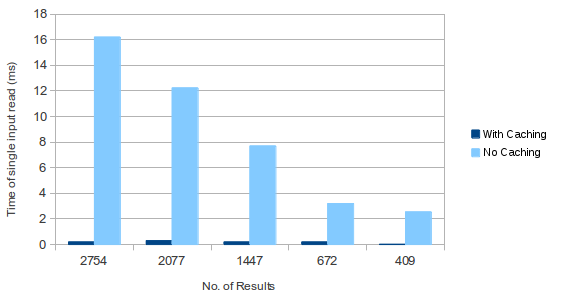
\includegraphics[width=0.8\textwidth]{MapIndexing}
\caption{Using Map to Cash the Input Geometry: Performance Effect}
\label{figMap}
\end{figure}

\subsection{Time Complexity}

There is no need to emphasize on importance of the role that indexing plays in query time and performance improvement. Here, we use real-world data to observe the effect of the currently implemented spatial index, followed by in depth looking at the implementation from other perspectives, aiminging to achieve better performance. This data is provided by University of Twente, Department of Geoinformation Processing [???] and holds some real information of geometries on earth, in \textit{GML 2.0} format. The original file based on one of the Netherlands' coordinate system (RD/NAP Amersfoort RD New) [???] is around 133.3 MB and have 12773 polygons inside 11886 multipolygons.
We run different queries on this database with and without spatial index to see time consumption dependency on the index structure. Moreover, queries have various number of results, to see also the trend changes concerning the number of outputs.
To start with, we take a look at the effect on index utilization in queries in comparison with queries using no spatial index. Figure~\ref{figIndexEfficiency} shows the effectiveness of index utilization.

 \begin{figure}
\centering
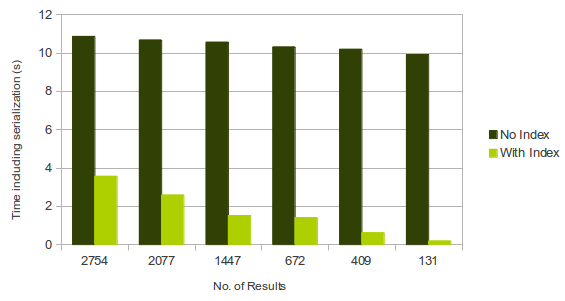
\includegraphics[width=0.8\textwidth]{IndexEfficiency}
\caption{Query Performance Improvement by Using Spatial Index}
\label{figIndexEfficiency}
\end{figure}

As it can be seen in this Figure, the query time when spatial index is not used, is fixed for every query regardless of the number of results. It means, no matter how big the output is, it takes the same time. As mentioned before, this is because of the fact that for each query, the whole file is scanned and analyzed. In contrast, queries using spatial index relatively take more time as the number of output objects goes higher. It confirms that filtering approach are going in the right direction, but the performance still is not satisfying. Thus, we need to investigate more ways to improve it.
By monitoring the times consumed by different part of a query, we discovered that \textit{JTS GMLReader} functions also takes considerable amount of time (see Figure??????). It should be mentioned that up to this point \textit{JTS GMLReader} class is being used to read and parse the geometries from GML and convert them to \textit{JTS} geometries.  

(make a chart to show the bigness of the reader time) ?????????????

Regarding the geometry reading process in \textit{JTS}, shown in Figure ?????, it seemed that direct parsing approach might declines the query time. Thus, we implemented a custom GML reader class to immediately parse the GML elements into \textit{JTS} geometries. As it was supposed, reading time drastically reduced by using the new functions. Figure … represents the time efficiencies.

\begin{figure}
\centering
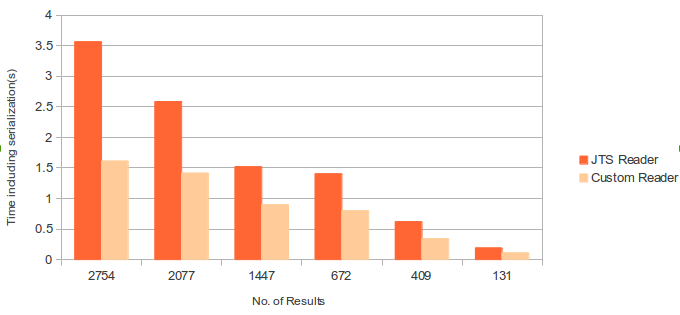
\includegraphics[width=0.8\textwidth]{GmlReader}
\caption{Custom GMLReader vs. JTS GMLReaer}
\label{figGmlReader}
\end{figure}


To achieve better performance, a deeper look at the different parts of a query will help to find the points to concentrate more. Suppose we run the query below,

\begin{verbatim}
let $a:= <gml:Polygon> … </gml:Polygon>
return ( geo-index:filter("DB", $a) [geo:intersects( . , $a)]
\end{verbatim}

The total query time will be divided into the following parts,

\begin{itemize}
\item reading the input geometry \textit{a}
\item filtering the geometries by \textit{filter} function 
\item reading the filtered geometries from the database
\item apply intersect operation on each pair of input geometry and selected geometries.
\end{itemize}

To follow the aim in this stage, we examine each part separately. Figure~\ref{figDetailedTiming} shows the time taken by the mentioned functions. It could be seen, that the biggest amount of time is still taken by reading process. Even the single reading of the input geometry seems to be expensive. Hence, the reading function should be examined more in detail.

\begin{figure}
\centering
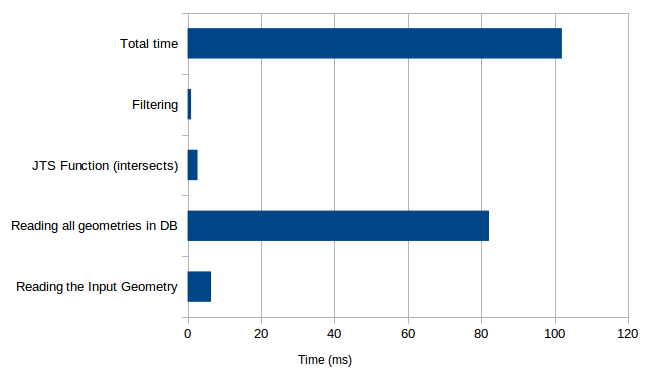
\includegraphics[width=0.8\textwidth,height=0.25\textheight]{detailedTiming}
\caption{Detaled Timing in Index Structure}
\label{figDetailedTiming}
\end{figure}


We have used java profiling to get more precise information. The first few methods in profile output with the highest percentage of time occupation, ordered from most-used to least-used, are listed in the following,

\begin{verbatim}
rank   	self  		accum     count   	method
   1 	6.95%  		6.95%      94  	  org.basex.util.Token.split
   2  	5.33% 		12.28%     72 	  org.expath.ns.GmlReader.createPolygon
   3  	4.59% 		16.86%     62  	  org.basex.util.Token.split
   4  	4.22% 		21.08%     57  	  org.basex.query.func.JavaModuleFunc.eval
   5  	3.55% 		24.63%     48  	  org.expath.ns.Geo.geo
   6  	3.18% 		27.81%     43 	  org.basex.util.Token.split
   7 	3.03% 		30.84%     41  	  org.basex.util.Token.split
   8  	2.96% 		33.80%     40  	  org.basex.util.Token.split
   9  	2.74% 		36.54%     37  	  org.expath.ns.Geo.geo
\end{verbatim} 

As the profile output indicates, the call for function \textit{split} consumes the greatest amount of time. Besides, \textit{createPolygon} and \textit{geo} functions, all used in \textit{GmlReader} class are expensive. Therefore, these functions should be focused in performance tuning, if this approach would be taken.
%TODO\CONTINUE

\subsection{Conclusion}


\newpage
\section{BaseX vs MongoDB}
\label{s.mongo}
%TODO:Complete

MongoDB geospatial features are explained before in \ref{mongo}. In this section we will have a more detailed overview of these functionalities and a general comparison between BaseX and MongoDB. However these two systems follow distinct approaches, it would be beneficial to review MongoDB as a rather new, recently developed, and widely used database system and among the few NOSQL systems providing geospatial features. Here we will mainly see differences between these systems, particularly in performance of the same features, and in which way we could improve the geospatial querying performance in BaseX. 


\subsection {MongoDB General Geospatial Features}
As mentioned before, \textit{GeoJSON} is the format supported by MongoDB geospatial operators. GeoJSON is a human-readable encoding format for representing the geographical features, using JSON standard. GeoJSON involve an object that could be a geometry, a Feature, or a collection of Features. \textit{Feature} is a geometry with more properties and \textit{FeatureCollection} conains a set of Features. Geometries are \textit{Point}, \textit{LineString}, \textit{Polygon}, \textit{MultiPoint}, \textit{MultiLineString}, \textit{MultiPolygon}, and \textit{GeometryCollection}. Bellow is a GeoJSON file with a \textit{FeatureCollection} object,

\begin{verbatim}
{
  "type": "FeatureCollection",
  "features": [
    {
      "type": "Feature",
      "geometry": {
        "type": "Point",
        "coordinates": [102.0, 0.5]
      },
      "properties": {
        "prop0": "value0"
      }
    },
    {
      "type": "Feature",
      "geometry": {
        "type": "LineString",
        "coordinates": [
          [102.0, 0.0], [103.0, 1.0], [104.0, 0.0], [105.0, 1.0]
        ]
      },
      "properties": {
        "prop1": 0.0,
        "prop0": "value0"
      }
    }
  ]
}
\end{verbatim}

MongoDB supports Point, LineString, and Polygon in \textit{WGS84} coordinate system, the latest revision of \textit{WGS}. \textit{WGS84} is used to represent the geospatial information on the Earth. Therefore, geometric calculations are provided on spherical space. As mentioned in Section \ref{mongo}, the geo spatial queries could be selected using \textit{geoIntersects}, \textit{geoWithin}, \textit{near}, and \textit{nearSphere}. In addition, there are geometry specifiers which are used to define geometries in query conditions. As an example, in a query to find the all geometries within a circular area, \textit{\$center} or \textit{\$centerSphere} is used to specify the circle, or \textit{\$maxDistance} determines the maxmimum distance from a point to be examined, in order to find geometries up to this distance. Geometry specifires are limited to, \textit{\$geometry}, \textit{\$maxDistance}, \textit{\$center}, \textit{\$centerSphere}, \textit{\$box}, and \textit{\$polygon}.

 
Geospatial index structure are available to be applied in queries based on the use case. That means, \textit{geoIntersects}, \textit{geoWithin} could be done with or without spatial index and \textit{near} or \textit{nearSphere} queries need geospatial index to be executed.
%TODO-continue

\subsection{Querying the Databases}

To analyse and compare the databases behaviour, designing the same test queries on the identical dataset is the most straight approach. Having some structural changes based on the MongoDB geospatial features and properties, the old Netherland data used to test BaseX \textit{Geo Module} is utilized. A brief explanation of the changes is provided here to clarify the rules and limitaions. The main change was to either remove \textit{MultiPolygon}s from the dataset or transforming them to a set of distinct Polygons, since this geometry is not supported in MongoDB. Besides, the coordinate system has to be changed to \textit{WGS84}. At the end, there are 12773 \textit{Polygon}s and no \textit{MultiPolygon} in the data file. The whole queries used before to test BaseX have to be repeated again, since the geometries have changed in database and the results would be different. 

To start with, the \textit{GeoJSON} file containing the geometries is imported into MongoDB, using \textit{java API}. It could be done also through Mongo Shell with appropriate \textit{mongoimport} command. There are some limitations to consider when using geo spatial features in MongoDB. The main one is the document size limitation in a collection. Document in MongoDB applies to the sets of key-values and would repeat through the whole collection. In other words, a collection in a database could be correspond with a table and documents involved documents as records. To successfully import a document into a collection, it  should be smaller than 16MB [ref to website]. Since it is normal to have large geometries in real geographic data files, this might appear as a problem. Aother limitation is that the z coordinate is not supported in MongoDB and no error massage will be shown when a coordinate contains third value as z coordinate. Instead, those geometries will not be processed. Additionally, geometries, like \textit{MultiPoint}, \textit{MultiLineString}, and \textit{MultiPolygon}, which are not supported in MongoDB  will be skipped in queries, without any error massage. 

In addition to the abovementioned limitations, importing a \textit{JSON} file into MongoDB should contain individual Features or geometries as bellow, 
 
\begin{verbatim}
    {
      "type": "Feature",
      "geometry": {
        "type": "Point",
        "coordinates": [102.0, 0.5]
      },
      "properties": {
        "prop0": "value0"
      }
    },
    {
      "type": "Feature",
      "geometry": {
        "type": "LineString",
        "coordinates": [
          [102.0, 0.0], [103.0, 1.0], [104.0, 0.0], [105.0, 1.0]
        ]
      },
      "properties": {
        "prop1": 0.0
      }
    }, 
    { ... }, ..., { ... }
\end{verbatim}

Since a \textit{FeatureCollection} contains the whole objects inside and is considered as one object, it might be bigger than 16MB and should not choosed as the imported file structure. This structure for the above file will be as following,
\begin{verbatim}
{
 "type": "FeatureCollection",
 "crs": 
    { "type": "name", "properties": { ... } },
                                                                                
 "features": [
     {
       "type": "Feature",
       "geometry": { ... },
       "properties": { ... }
     },
     {
       "type": "Feature",
       "geometry": { ... },
       "properties": { ... }
     }, 
     { ... } , { ... }
 ]
}
\end{verbatim}

%TODO:explain about the query difficulties and aggregation of the above structure
After importing the file, we have tried to examine the common features, i.e., intersection, within and near functionalities, in both databases.
The sample queries are applied to the databases either with using geospatial index or without any, regarding some limitations that database functionalities may define, like \textit{near} queries in MongoDb that definately need the geospatial index as mentioned or using the \textit{distance} function to find the near geometries in BaseX in which the current index structure is not applicable.
The following queries find the intersecting geometries with the given one in \textit{BaseX} and \textit{MongoDB},

\begin{itemize}
\item \textit{BaseX}:
\begin{verbatim}
import module namespace geo = "http://expath.org/ns/Geo";
declare namespace gml="http://www.opengis.net/gml";
let $a:= <gml:Polygon>
              <gml:outerBoundaryIs>
                <gml:LinearRing>
                  <gml:coordinates decimal="." cs="," ts=" ">
                  6,52.6 6.1,52.6 6.1,53 6,53 6,52.6
                  </gml:coordinates>
                </gml:LinearRing>
              </gml:outerBoundaryIs>
            </gml:Polygon>
for $b in //gml:Polygon 
return if (geo:intersects( $a, $b)) then $b else ()
\end{verbatim}
\item \textit{MongoDB}: 
\begin{verbatim}
db.places.find( { geometry :
                  { $geoIntersects :
                    { $geometry :
                      { type : "Polygon" ,
                        coordinates:[[[6,52.6],[6.1,52.6],
                        	    [6.1,53],[6,53],[6,52.6]]]
                } } } } )
\end{verbatim}
\end{itemize}
Similar queries are designed to check the other function. Here we skip the queries and directly go to the results. To check the profiling in MongoDB, query plan information, such as the index type, the query time, scanned objects, and more \textit{\$explain} operator could be specified either in the forms,
\begin{verbatim}
db.collection.find()._addSpecial( "$explain", 1 )
db.collection.find( { $query: {}, $explain: 1 } )
\end{verbatim}
 or 
 \begin{verbatim}
 db.collection.find().explain().
 \end{verbatim}
 
Bellow the profile of a sample query is shown,

\begin{verbatim}
"cursor" : "BasicCursor",
"isMultiKey" : false,
"n" : 2756,
"nscannedObjects" : 12773,
"nscanned" : 12773,
...
...
"millis" : 43907,
...
"server" : "MongoServer"
\end{verbatim}

In the provided information, number of the results and the query time is implied in \textit{n} and \textit{millis} elements respectively. \textit{cursor} specifies the type of the cursor used by the operation. Here, \textit{BasicCursor} indicates that the query is only performing the a normal scan to find the results and typical cursor is used which reads the documents in natural order. That is, no index is used for this operation and the whole data is scanned in the original order. If a geospatial index \textit{2dsphere} is used, the cursor type will be \textit{S2Cursor}. \textit{n} reflects the number of geometries that match the query condition (i.e. the number of items on the cursor). \textit{nscanned} is the number of documents or index entry in the range (in case that index is used), scanned for this operation and \textit{nscannedObjects} is the number of the documents scanned in this query to get the results. In queries which the index structure is not used, as in the above sample, these two numbers will be equal. Otherwise, \textit{nscannedObjects} may be lower, as shown in the following query plan which uses \textit{2dsphere} index. 

\begin{verbatim}
"cursor" : "S2Cursor",
"isMultiKey" : true,
"n" : 2756,
"nscannedObjects" : 3370,
"nscanned" : 36941,
...
\end{verbatim}

In other words, nscanned >= nscannedObjects >= n always. Ofcourse, the most optimum state is where scanned = nscannedObjects = n and it could be reached with compound indexes and rephrasing the query statement in some cases as well.
%TODO mesal for optimization from: http://java.dzone.com/articles/optimizing-mongodb-compound

Having the same queries, Figure ~\ref{figBXvsMongoNoIndexIntersects} shows the timing of various queries without using any geospatial index in both databases. As it could be seen, the timing of all queries are more or less the same, since the whole data is typically scanned when no index is used. It is also obvious from the query plan in MongoDB which specifies the cursor type, number of index keys scanned (nscsnned), and number of documents scanned to get the result (nscsnnedObjects),
\begin{verbatim}
...
"n" : 12773,
"nscannedObjects" : 12773,
"nscanned" : 12773,
...
\end{verbatim}

\begin{figure}
\centering
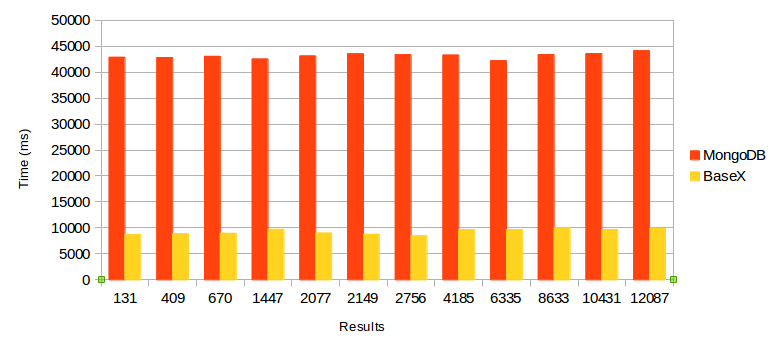
\includegraphics[width=\textwidth,height=0.25\textheight]{BXvsMongo-NoIndex-Intersects}
\caption{Query Timing of \textit{intersect} Operation without Spatial Index}
\label{figBXvsMongoNoIndexIntersects}
\end{figure}

This process is continued by applying the geospatial index. In MongoDB there are two choices for using geospatial index, \textit{2d} for data expressed in legacy coordinate pairs and \textit{2dsphere} for both \textit{GeoJSON} data objects and legacy coordinate pairs. We use \textit{2dsphere} which fits to our sample data, via the following shell command,

\begin{verbatim}
db.Collection.ensureIndex({geometry:"2dsphere"})  
\end{verbatim}

The same step is also taken in BaseX since the index structure can be used in both intersection and within functions. Running again the same queries using a geospatial index, supposedly gives declined query times (see Figure~\ref{figBXvsMongoIndexIntersects}). As explained in Section~\ref{s.basex}, in BaseX index is apllied through the \textit{filter} function, while MongoDB follows another approach. MongoDB applies the index in casual query formats after executing the above-mentioned command and there is no need to change the queries in general. 


\begin{figure}
\centering
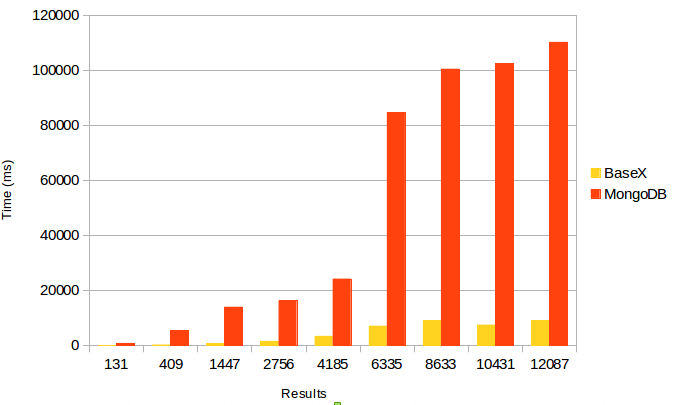
\includegraphics[width=0.7\textwidth]{BXvsMongo-Intersects-Index}
\caption{Query Timing of \textit{intersect} Operation with Spatial Index}
\label{figBXvsMongoIndexIntersects}
\end{figure}

Besides, the search for the geometries within an input area is done in the same way and the timings are shown in Figure~\ref{figBXvsMongoIndexWithin}. It can be seen that the queries with smaller number of returned geometries have better performane in MongoDB. Although it seems a positive point to return the big numbers of result in as shorter time as possible, considering smaller returned numbers of results is of greate importance for us, since these queries are more common in real-world usecases.

% TODO
%\begin{figure}
%\centering
%\includegraphics[width=0.7\textwidth]{BXvsMongo-Within-Index}
%\caption{Query Timing of \textit{intersect} Operation with Spatial Index}
%\label{figBXvsMongoIndexIntersects}
%\end{figure}

The next wiedly used type of query is finding the near places or geometries up to a distance from a specific point. It could be also expressed as finding the geometries inside a polygon or specifically a circle with the distance value as the radius lenght. This feature is provided in MongoDB via \textit{near} and \textit{nearSphere} operators which simply get the reference point and the disance and hereafter returns the whole geometries in the specified distance from the point. In the following we have provided a sample query of this feature. Both near operators nead a geospatial index, either \textit{2d} or \textit{2dsphere}. A specific distance in meter could be defined as a condition to filter those geometries included to this distance. 

\begin{verbatim}
db.collection.find({{geometry:
                         {$nearSphere:
                            {$geometry:
                               {type:"Point", coordinates:[4.5,51.95]}, 
                             $maxDCistance : 100}
                         }
                     }
                   })
\end{verbatim}


BaseX \textit{Geo Module} could provide this feature via \textit{distance} or combination of \textit{buffer}, \textit{within} functions. In Both cases, meter as the unit for distance specification works for the projected coordinate systems\cite{}. In a projected coordinate system all the areas, lengths, and angels are defined on a flat two-dimensional space. In such a system, the user is provided with this feature, using the above-mentioned functions, as the following example,

\begin{verbatim}
import module namespace geo = "http://expath.org/ns/Geo";
declare namespace gml="http://www.opengis.net/gml";
let $a:= <gml:Point>
              <gml:coordinates>
               4.5,51.95 
               </gml:coordinates>
            </gml:Point>
for $b in //gml:Polygon 
return if (geo:distance( $a, $b) le 500) then $b else ()
\end{verbatim}


For the data provided in a geographic coordinate system\cite{}, calculations do not work with metric values. A geographic coordinate system, such as \textit{WGS89}, defines the areas and locations in a three-dimensional spherical space. The \textit{distance} function in BaseX will get the distance in the same coordinate system which the data are provided and ofcourse it is not in meters. In other words, there is not a specific units for existing \textit{Geo Module} and the calculations are based on the coordinate system of the data, and the distance between every two geometries in any coordinate system is calculated by the distance rules and formulas on the flat space. ???????????????????
As a consequence, to find a distance on earth we will need to work in a metric coordinate system. An idea could be to convert the geometry to a projected coordinate system. Then, to spacify the buffer of converted geometry up to the defined distance in meter, in the same metric system and convert the buffer back to the original geographic coordinate system to find the all geometries within this area. In this way we could benefit from the geospatial index structure, via the \textit{within} function........................................
This procedure be expressed as bellow, using the current \textit{buffer} and \textit{within} functions, 

% TODO: indention
\begin{verbatim} 
	within(geometry,transform(buffer(
				transform(myPoint_in_wgs84, other_metric_cs),
			  	500),
		wgs84))
\end{verbatim}


??????????As shown in Figure~\ref{figBXvsMongoNear}, performance of finding near geometries in MongoDB gives a better result............
This is also obvious from the timing results in BaseX as every number of results is returned more or less in the same time.

?????????? figure for converion method in BX


\begin{figure}
\centering
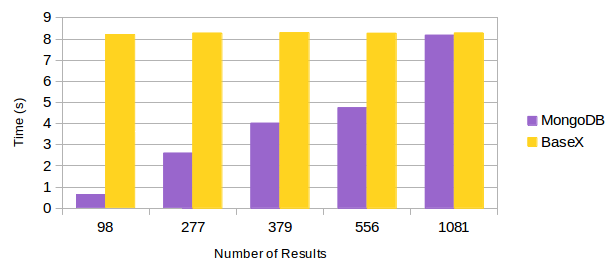
\includegraphics[width=0.7\textwidth]{BXvsMongoNear.png}
\caption{Query Timing of \textit{near} Operation}
\label{figBXvsMongoNear}
\end{figure}


Opening the index into main memory ????????????????????


\subsection{Updating a Database}

Updating a database as a significant interaction supplied by the database system generally comprise three different operation: insert, delete, and modify. In addition to the whole issues related to database update on disk and memory, reconstructing the indexes is also of great importance. That is, since the index is constructed based on the old structure and values, hence, the updated database needs a new index. 

Currently in BaseX, updating is not applied to the geospatial index after the database update operations. It means, the STRTree do not get updated automatically and accordingly, the geospatial index has to be rebuilt manually, which would cause redundant constructions and consequently, worse performance. Here, we see how it could effect the updating performance, comparing with MongoDB, since it manages to rebuild the index in the updating process.

Considering the manual update of the geospatial index in BaseX, to evaluate an update process by which the database and the index is updated, reindexing time have to be considered. This implies, the index creation time plus reopeneing the index file into the main memory should be included in the evaluation. In MongoDB, we have concentrated on updating operations using the geo spatial index, while the consumed time also contains the index structure updating. 


As shown in Figure~\ref{figBXvsMongoUpdate}, performance of all update operations in MongoDB are obviously better. As mentioned before, reindexing causes a huge growth in time, which individually takes the greatest amount of total time (See Figure~\ref{figBXUpdate}).  ?????????????????
 


\begin{figure}
\centering
\subfigure{
	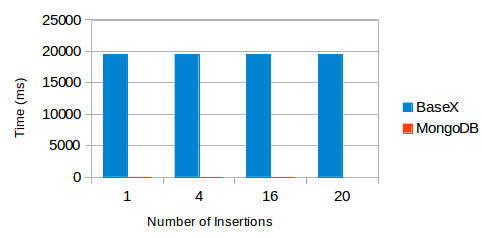
\includegraphics[width=0.47\textwidth]{BXvsMongo-Insertion.png}
	\label{figBXvsMongoInsert}
}
\centering
\subfigure{
	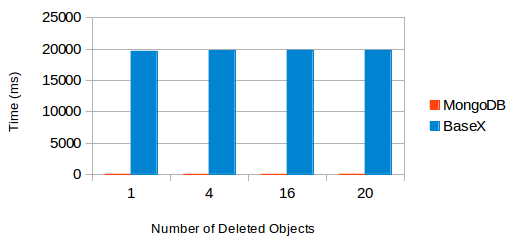
\includegraphics[width=0.47\textwidth]{BXvsMongo-Deletion.png}
	\label{figBXvsMongoDelete}
}
\subfigure{
	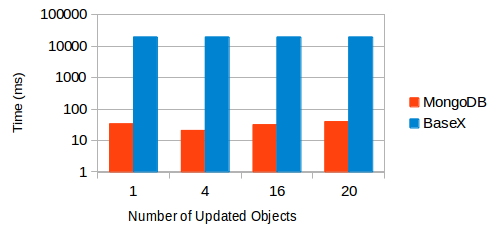
\includegraphics[width=0.5\textwidth]{BXvsMongo-Update.png}
	\label{figBXvsMongoModify}
}
\caption{Performance of different update operations in BaseX and MongoDB.}
\label{figBXvsMongoUpdate}
\end{figure}


\begin{figure}
\centering
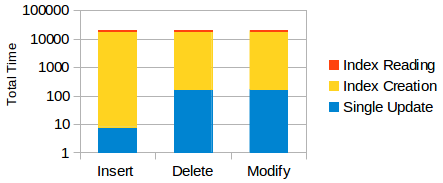
\includegraphics[width=0.5\textwidth]{BXUpdate.png}
\caption{Time consumtion percentage of different tasks in update operations in BaseX.}
\label{figBXUpdate}
\end{figure}

\newpage
\subsection{Conclusion}


\newpage
\section{Future Work}
\label{s.future}
\newpage
\bibliographystyle{unsrt}
\bibliography{refs}

\end{document}
